\documentclass{beamer}

\usepackage{float}
\usepackage{verbatim}
\usepackage{moreverb}
\usepackage{listings}
\usepackage{minted}
\usepackage{upquote} % this makes backticks show correctly in minted

\let\verbatiminput=\verbatimtabinput
\def\verbatimtabsize{4\relax}

\graphicspath{{./images/}}

\begin{document}
\title{A Verilog Primer}
\subtitle{An Overview of Verilog for Digital Design and Simulation}
\author{John Wright \and Vighnesh Iyer}
\institute{Department of Electrical Engineering and Computer Sciences\\
	College of Engineering, University of California, Berkeley}
\date{}

\frame{\titlepage}

% Topics Left to Add:
%	Finite State Machines (this should probably be another presentation)
%	Simulation Verilog constructs (this should also be another presentation, the initial block slides provide a good but brief background)
%	A complete Verilog design example of some block + its verification (binary search module which clocks in 32 32-bit numbers in ascending sorted order and will then clock in a 32-bit number to search for using binary search. The module will then return the index the number is found and a flag to indicate if the number was found in the list.)
%	General digital design/architecture techniques (synchronous/asynchronous resets, FIFOs, pipelining, system buses, off-chip communication protocols, clock-domain crossing) (this is for another presentation or document)

\begin{frame}{What is Verilog?}
	\begin{columns}
		\begin{column}{0.5\textwidth}
			\begin{block}{Visual Circuit Design}
				Digital circuits can be designed by laying out circuit elements. This was done in CS 61C. Schematic entry.
			\end{block}
			\begin{block}{Logisim}
				\centerline{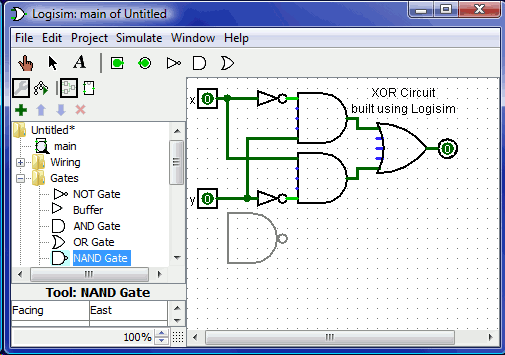
\includegraphics[width=\textwidth]{logisim_screenshot.png}}
			\end{block}
		\end{column}
		\begin{column}{0.5\textwidth}
			\begin{itemize}
				\item Verilog is a HDL (hardware definition language) that can describe digital circuits with C-like syntax.
				\item Defines circuits at the RTL (register-transfer level) of abstraction
				\item The circuit on the left could be written in Verilog as \texttt{assign output = x \^{} y}
				\item ASIC or FPGA toolchains translate Verilog to a gate-level netlist
			\end{itemize}
		\end{column}
	\end{columns}
\end{frame}

\begin{frame}[fragile]{Verilog Modules}
	\begin{itemize}
		\item Modules are the building blocks of Verilog designs. They are a means of abstraction and encapsulation for your design.
		\item A module consists of a port declaration and Verilog code to implement the desired functionality.
		\item Modules should be created in a Verilog file (.v) where the filename matches the module name (the module below should be stored in full\_adder.v)
	\end{itemize}
	
\begin{minted}[fontsize=\scriptsize]{verilog}
module full_adder (input x, input y, input cin, output s, output cout);
endmodule
\end{minted}
	\begin{figure}[H]
	\centering
	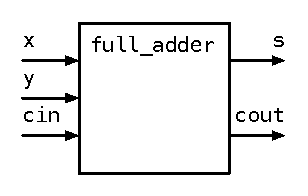
\includegraphics[height=3cm]{full_adder.pdf}
	\end{figure}
\end{frame}

\begin{frame}[fragile]{Verilog Module I/O Ports}
	\begin{itemize}
		\item Ports allow communication between a module and its environment
		\item Each port has a name and a type
		\begin{itemize}
			\item input
			\item output
			\item inout
		\end{itemize}
		\item Ports for a module are declared in the port declaration
	\end{itemize}
\begin{minted}[fontsize=\scriptsize]{verilog}
module full_adder (input x, input y, input cin, output s, output cout);
	// Verilog code here has access to inputs
	// Verilog code here can drive outputs
endmodule
\end{minted}
\end{frame}

\begin{frame}{The Top-Level Module}
	\begin{itemize}
		\item Every Verilog design has a top-level module which sits at the highest level of the design hierarchy
		\item The top-level module defines the I/O for the entire digital system
		\item All the modules in your design reside inside the top-level module
	\end{itemize}
	\begin{figure}
	\centering
	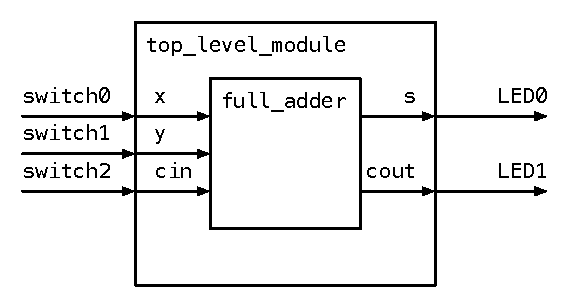
\includegraphics{top_level.pdf}
	\end{figure}
\end{frame}

\begin{frame}[fragile]{Verilog Module Instantiation}
	\begin{itemize}
		\item Modules can be instantiated inside other modules. The syntax used is \small \texttt{<module name> <instance name> (.port0(wire), .port1(wire), ...)}\normalsize
	\end{itemize}
\begin{minted}[fontsize=\scriptsize]{verilog}
module top_level (input switch0,
                  input switch1,
                  input switch2,
                  output LED0,
                  output LED1);
	full_adder add (
		.x(switch0),
		.y(switch1),
		.cin(switch2),
		.s(LED0),
		.cout(LED1)
	);
endmodule
\end{minted}
\end{frame}

\begin{frame}[fragile]{Wire Nets}
	\begin{itemize}
		\item Wires are analogous to wires in a circuit you build by hand; they are used to transmit values between inputs and outputs. Declare wires before they are used.
	\end{itemize}
\begin{minted}{verilog}
wire a;
wire b;
\end{minted}

	\begin{itemize}
		\item The wires above are scalar (represent 1 bit). They can also be vectors:
	\end{itemize}
\begin{minted}{verilog}
wire [7:0]  d;  // 8-bit wire declaration
wire [31:0] e; // 32-bit wire declaration
\end{minted}
\end{frame}

\begin{frame}[fragile]{Multi-bit Nets}
	\begin{itemize}
		\item We can declare signals that are more than 1 bit wide in Verilog
		\item Use the syntax \texttt{[MSB bit index : LSB bit index]} before a signal name to declare its bit-width
		\item When connecting multi-bit inputs or outputs to another module, the bit-widths of the signals need to match!
	\end{itemize}
\begin{minted}[fontsize=\scriptsize]{verilog}
module two_bit_adder (input [1:0] x, input [1:0] y, output [2:0] sum);
	wire [1:0] partial_sum;
	wire carry_out;
endmodule
\end{minted}
\end{frame}

\begin{frame}[fragile]{Structural Verilog with Gate Primitives}{Gate-Level Circuit Construction}
	\begin{itemize}
		\item The following gate primitives exist in Verilog: and, or, xor, not, nand, nor, xnor. In general, the syntax is:
	\end{itemize}
\begin{minted}[fontsize=\scriptsize]{verilog}
<operator> (output, input1, input2); // for two input gate
<operator> (output, input); // for not gate
\end{minted}

Example of Verilog that implements the Boolean equation $f = a + b$:

\begin{minted}[fontsize=\scriptsize]{verilog}
wire a, b, f;
or (f, a, b);
\end{minted}
\end{frame}

\begin{frame}{Designing the Full Adder}{Gate-Level Circuit}
\begin{figure}[H]
\centering
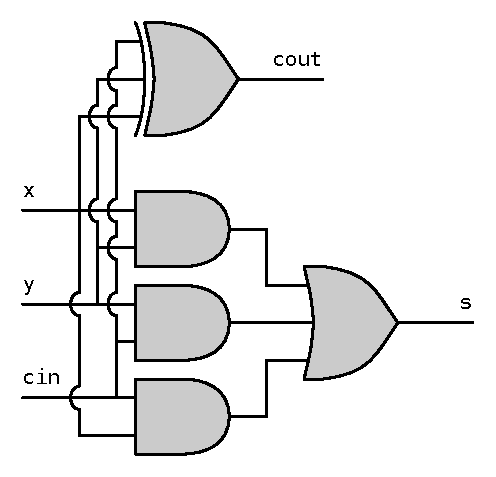
\includegraphics{full_adder_gates.pdf}
\end{figure}
\end{frame}

\begin{frame}[fragile]{Designing the Full Adder}{Using Structural Verilog}
\begin{minted}[fontsize=\scriptsize]{verilog}
module full_adder (input x, input y, input cin, output s, output cout);
	xor(cout, x, y, cin);
	
	wire and_x_y;
	wire and_y_cin;
	wire and_x_cin;
	and (and_x_y, x, y);
	and (and_y_cin, y, cin);
	and (and_x_cin, x, cin);
	or (s, and_x_y, and_y_cin, and_x_cin);
endmodule
\end{minted}
\end{frame}

\begin{frame}{Behavioral Verilog}{Letting the tools translate RTL to gates}
	\begin{itemize}
		\item The full adder using structural Verilog was a pain to write, but you will never have to write it that way!
		\item Behavioral Verilog constructs allow you to describe what you want a circuit to do at the RTL level of abstraction
		\item The FPGA or ASIC toolchain will translate the Verilog code to the FPGA or ASIC primitives that implement your circuit description
		\item Verilog's gate primitives are typically not used in design
	\end{itemize}
\end{frame}

\begin{frame}[fragile]{Assign Statements}
	\begin{itemize}
		\item Wires can be assigned to logic equations, other wires, or operations performed on wires
		\item This is accomplished using the 'assign' statement
		\item The left argument of the assign statement must be a wire, and cannot be an input wire
		\item The right argument of the assign statement can be any expression created from Verilog operators and wires
	\end{itemize}
\begin{minted}{verilog}
module copy (input a, output b);
	assign b = a;
endmodule
\end{minted}
\end{frame}

\begin{frame}[fragile]{Verilog Operators}
	\begin{itemize}
		\item Verilog contains operators that can be used to perform arithmetic, form logic expression, perform reductions/shifts, and check equality between signals.
	\end{itemize}
	\begin{center}
	\begin{tabular}{l | l | l}
		Operator Type & Symbol & Operation Performed \\ \hline
		Arithmetic & \texttt{+} & Add \\ \hline
		& \texttt{-} & Subtract \\ \hline
		& \texttt{*} & Multiply \\ \hline
		& \texttt{/} & Divide \\ \hline
		& \texttt{\%} & Modulus \\ \hline
		Logical & \texttt{!} & Logical negation \\ \hline
		& \texttt{\&\&} & Logical and \\ \hline
		& \texttt{||} & Logical or \\ \hline
	\end{tabular}
	\end{center}
\end{frame}

\begin{frame}[fragile]{Verilog Operators Cont.}
	\begin{center}
		\begin{tabular}{l | l | l}
			Operator Type & Symbol & Operation Performed \\ \hline
			Relational & \texttt{>} & Greater than \\ \hline
			& \texttt{<} & Less than \\ \hline
			& \texttt{>=} & Greater than or equal \\ \hline
			& \texttt{<=} & Less than or equal \\ \hline
			Equality & \texttt{==} & Equality \\ \hline
			& \texttt{!=} & Inequality \\ \hline
			Bitwise & \texttt{\~} & Bitwise negation \\ \hline
			& \texttt{\&} & Bitwise AND \\ \hline
			& \texttt{|} & Bitwise OR \\ \hline
			& \texttt{\^} & Bitwise XOR \\ \hline
		\end{tabular}
	\end{center}
	Reduction operators also exist for AND, OR, and XOR that have the same symbol as the bitwise operators.
\end{frame}

\begin{frame}[fragile]{Verilog Operators Cont.}{Shifts, Concatenation, Replication, Indexing multi-bit wires}
	\begin{center}
		\begin{tabular}{l | l | l}
			Operator Type & Symbol & Operation Performed \\ \hline
			Shift & \texttt{<<} & Shift left logical \\ \hline
			& \texttt{>>} & Shift right logical \\ \hline
			& \texttt{<<<} & Arithmetic left shift \\ \hline
			& \texttt{>>>} & Arithmetic left shift \\ \hline
			Concatenation & \texttt{\{\}} & Join bits \\ \hline
			Replication & \texttt{\{\{\}\}} & Duplicate bits \\ \hline
			Indexing/Slicing & \texttt{[MSB:LSB]} & Select bits \\ \hline
		\end{tabular}
	\end{center}
\begin{minted}{verilog}
wire [7:0] d;
wire [31:0] e;
wire [31:0] f;
assign f = {d, e[23:0]}; // Concatenation + Slicing
assign f = { 32{d[5]} }; // Replication + Indexing
\end{minted}
\end{frame}

\begin{frame}[fragile]{Designing the Full Adder}{Using Behavioral Verilog}
\begin{minted}[fontsize=\scriptsize]{verilog}
module full_adder (input x, input y, input cin, output s, output cout);
	assign cout = x ^ y ^ cin;
	assign s = (x && y) || (x && cin) || (y && cin);
endmodule
\end{minted}
This is much better than the structural Verilog representation of a full adder! The Verilog synthesizer can take this opportunity to optimize logic expressions.
\end{frame}

\begin{frame}[fragile]{Designing an Adder}{Using Behavioral Verilog}

But it gets even better!

\begin{minted}{verilog}
wire operand1 [31:0];
wire operand2 [31:0];
wire result [32:0];
assign result = operand1 + operand2;
\end{minted}

We just described a 32-bit adder, but didn't specify the architecture or the logic! The Verilog synthesizer will turn the generalized adder into a FPGA specific netlist or an ASIC gate-level netlist.
\end{frame}

\begin{frame}[fragile]{Conditional Operator ?:}
	\begin{itemize}
		\item The conditional operator allows us to define if-else logic in an assign statement.
		\item Syntax: (condition) ? (expression if condition is true) : (expression if condition is false)
		\item Let's design a circuit that will output 0 if the two inputs are equal, output 1 if input a is less than input b, and output 2 if input a is greater than input b.
	\end{itemize}

\begin{minted}[fontsize=\scriptsize]{verilog}
module equality_checker(input a [31:0], input b [31:0], output c [1:0]);
	assign c = a == b ? 2'd0 : (a < b ? 2'd1 : 2'd2);
endmodule
\end{minted}
\end{frame}

\begin{frame}[fragile]{Verilog Literals}
	\begin{itemize}
		\item Verilog defines a particular way of specifying literals
		\item Syntax: [bit width]'[radix][literal]
		\item Radix can be d (decimal), h (hexadecimal), o (octal), b (binary)
		\item It is critical to always match bit widths for operators and module connections, do not ignore these warnings from the tools
	\end{itemize}
\begin{minted}{verilog}
2'd1 2-bit literal (decimal 1)
16'hAD14 16-bit literal (hexadecimal 0xAD14)
8'b01011010 8-bit literal (binary 0b01011010)
\end{minted}
\end{frame}

\begin{frame}{Verilog Macros}{Constant defines + Helper functions}
	\begin{itemize}
		\item Macros in Verilog are similar to macros available in C
		\item \texttt{\`{}include} is a preprocessor command to inject a Verilog source file at its location; often used to bring in a Verilog header file (.vh)
		\item \texttt{\`{}define <Constant Name> <Constant Value>} is used to declare a synthesis-time constant; use these instead of putting 'magic' values in code
		\item \texttt{\`{}define <Macro function name>(ARGS) <Function body>} is used to define a macro function that can generate code based on ARGS.
		\item \texttt{\`{}ifndef <NAME>, \`{}define <NAME>, \`{}endif} is a include guard (used similarly in C).
	\end{itemize}
\end{frame}

\begin{frame}[fragile]{Verilog Macros}{Example}
Inside constants.vh:
\begin{minted}[fontsize=\scriptsize, breaklines]{verilog}
`ifndef CONSTANTS // guard prevents header file from being included more than once
`define CONSTANTS

`define ADDR_BITS 16
`define NUM_WORDS 32
`define LOG2(x) \
	(x <= 2) ? 1 : \
	(x <= 4) ? 2 : \
	(x <= 8) ? 3 : \
	(x <= 16) ? 4 : \
	(x <= 32) ? 5 : \
	(x <= 64) ? 6 : \
	-1
`endif
\end{minted}
\end{frame}

\begin{frame}[fragile]{Verilog Macros}{Example Cont.}
Inside design.v:
\begin{minted}[breaklines]{verilog}
`include "constants.vh"
module memory (input [`ADDR_BITS - 1:0] address, output [`LOG2(`NUM_WORDS) - 1:0] data);

	// implementation
	
endmodule
\end{minted}
\end{frame}

\begin{frame}[fragile]{Reg Nets}
	Verilog has two types of net: \texttt{wire} and \texttt{reg}.
	Reg nets are required whenever a net must preserve state (i.e. in an always block).
	Wires are used for structural verilog (to connect inputs to outputs) and for continuous assignment.

\begin{minted}{verilog}
	reg x;
\end{minted}

\end{frame}

\begin{frame}[fragile]{Combinational Logic Blocks using always@(*)}
	Verilog allows more complex logic through the use of \texttt{always} blocks.
	Combinational logic (i.e. no state elements) can be written using \texttt{always@(*)}.
	The value inside the parentheses is called the sensitivity list.
	Using a \texttt{*} will tell the compiler to compute the sensitivity list automatically (recommended for combinational logic).

\begin{minted}{verilog}
	reg y;
	reg x;
	always@(*)
	begin
		x = ~y;
	end
\end{minted}

\end{frame}

\begin{frame}[fragile]{If-else statements}
	Like many programming languages, verilog includes \texttt{if-else} statements.
	These implicitly generate multiplexors in hardware.
	Multi-line code blocks require \texttt{begin} and \texttt{end} statements.

\begin{minted}{verilog}
	input w;
	input y;
	input x;
	reg [1:0] z;
	always@(*)
	begin
		if(x) begin
			z[0] = w;
			z[1] = y;
		end else begin
			z[0] = y;
			z[1] = x;
		end
	end
\end{minted}

\end{frame}

\begin{frame}[fragile]{Case statements}
	Like C, verilog supports case statements for generating multiplexor structures.

\begin{minted}{verilog}
	input [1:0] x;
	reg [1:0] y;
	always@(*)
	begin
		case(x)
		0: y = 2'd0;
		1: y = 2'd3;
		2: y = 2'd2;
		default: y = 2'd2;
		endcase
	end
\end{minted}

\end{frame}

\begin{frame}[fragile]{Non-Synthesizable Control Statements}
	WARNING: \texttt{for} and \texttt{while} loops can't be mapped to hardware!

	These statements are valid verilog (and can be simulated), but cannot be mapped to hardware.
	Generate statements (more later) are the appropriate use for \texttt{for} loops.
\end{frame}

\begin{frame}[fragile]{Avoiding Unintentional Latch Synthesis}
	Every signal should have a default value.
	Assigning a value to a reg only under given conditions will result in latch synthesis.

	For example, this code generates a latch:

\begin{minted}{verilog}
	input [1:0] x;
	reg [1:0] y;
	always@(*)
	begin
		if(x == 2'b10) begin
			y = 2'd3;
		end else if(x == 2'b11) begin
			y = 2'd2;
		end
	end
\end{minted}

\end{frame}

\begin{frame}[fragile]{Avoiding Unintentional Latch Synthesis}

	This code has a default value and will not generate a latch:

\begin{minted}{verilog}
	input [1:0] x;
	reg [1:0] y;
	always@(*)
	begin
		y = 2'b00;
		if(x == 2'b10) begin
			y = 2'd3;
		end else if(x == 2'b11) begin
			y = 2'd2;
		end
	end
\end{minted}

\end{frame}

\begin{frame}[fragile]{Synchronous Logic Blocks}

	Synchronous logic blocks are generated using special identifiers in the sensitivity list.
	Here we only want to update on the positive edge of the clock, so we use \texttt{posedge}.
	This will generate a synchronous circuit that increments \texttt{x} every clock cycle.

\begin{minted}{verilog}
	input clk;
	reg [1:0] x;

	always@(posedge clk)
	begin
		x <= x + 1;
	end
\end{minted}

\end{frame}

\begin{frame}[fragile]{Blocking vs Non-Blocking Assignments}
	What was up with the \texttt{<=} operator on the last slide?
	Verilog has two assignment operators: blocking (\texttt{=}) and non-blocking (\texttt{<=}).
	For the purposes of this class, always use blocking (\texttt{=}) for combinational logic and non-blocking (\texttt{<=}) for sequential logic.

\begin{minted}{verilog}
	input clk;
	reg [1:0] x;
	reg [1:0] next_x;

	always@(*)
	begin
		next_x = x + 1;
	end

	always@(posedge clk)
	begin
		x <= next_x;
	end
\end{minted}

\end{frame}

\begin{frame}[fragile]{localparam Declarations}
	Private module parameters are defined using the \texttt{localparam} directive.
	These are useful for constants that are needed only by a single module.

\begin{minted}{verilog}
	localparam coeff = 5;
	reg [31:0] x;
	reg [31:0] y;

	always@(*)
	begin
		x = coeff*y;
	end

\end{minted}

\end{frame}

\begin{frame}[fragile]{Wire vs. Reg}{What is a real register and what is just a wire?}
	Follow these rules to figure out when to use a wire and when to use a reg net type:
	\begin{itemize}
		\item If a signal needs to be assigned inside an always block, it must be declared as a reg.
		\item If a signal is assigned using a continuous assignment statement, it must be declared as a wire.
		\item By default module input and output ports are wires; if any output ports are assigned in an always block, they must be explicitly declared: \texttt{output reg <signal name>}
	\end{itemize}
	
	How to know if a net represents a register or a wire.
	\begin{itemize}
		\item A wire net always represents a combinational link
		\item A reg net represents a wire if it is assigned in an always @ (*) block
		\item A reg net represents a register if it is assigned in an always @ (posedge/negedge clock) block
	\end{itemize}
\end{frame}

\begin{frame}[fragile]{Code Generation with for-generate loops}
	Generate loops are used to iteratively instantiate modules.
	This is useful with parameters (next slide) or when instantiating large numbers of the same module.

	\begin{minted}[fontsize=\scriptsize]{verilog}
	wire [3:0] a, b;
	genvar i;

	core_inst firstone (1'b0, a[i], b[i]);

	// programmatically wire later instances
	generate
		for (i = 1; i < 4 ; i = i + 1) begin:nameofthisloop
			core core_inst (a[i], a[i-1], b[i]);
		end
	endgenerate
	\end{minted}

\end{frame}

\begin{frame}[fragile]{Verilog Module Parameterization}
	Verilog modules may include parameters in the module definition.
	This is useful to change bus sizes or with generate statements.
	Here we define and instantiate a programmable-width adder with a default width of 32.

	\begin{minted}[fontsize=\scriptsize]{verilog}
	module adder #(parameter width=32)
		(input [width-1:0] a,
		 input [width-1:0] b,
		 output [width:0] s);
		s = a + b;
	endmodule

	module top();
		localparam adder1width = 64;
		localparam adder2width = 32;
		reg [adder1width-1:0] a,b;
		reg [adder2width-1:0] c,d;
		wire out1;
		wire out2;
		adder #(.width(adder1width)) adder64 (.a(a), .b(b), .s(out1));
		adder #(.width(adder2width)) adder32 (.a(c), .b(d), .s(out2));
	endmodule
	\end{minted}

\end{frame}

\begin{frame}{Multidimensional Nets in Verilog}
	\begin{itemize}
		\item It is often useful to have a net organized as a two-dimensional net to make indexing easier; this is particularly useful in any memory structure.
		\item Syntax: \texttt{reg [M:0] <netname> [N:0]}
		\item The line above creates a net called \texttt{<netname>} and describes it as an array of (N+1) elements, where each element is a (M+1) bit number.
	\end{itemize}
\end{frame}

\begin{frame}{Memory Module Design Example}{High-Level Spec}
	Let's design a memory module with the following capabilities.
	\begin{itemize}
		\item Parameterized number of bits per word
		\item Parameterized number of words
		\item Asynchronous reads (as soon as an address is driven into the memory, after a combinational delay, the data at the address will come out of the memory)
		\item Synchronous writes (at a rising clock edge, if the write signal is high, write the memory with the contents on the data input line and at the address provided as input)
	\end{itemize}
\end{frame}

\begin{frame}[fragile]{Memory Module Design Example}{Module + Port Declaration}
\begin{minted}{verilog}
module memory #(
	parameter BITS_PER_WORD = 32, 
	parameter NUM_WORDS = 128)(
	input clk,
	input [`LOG2(NUM_WORDS) - 1 : 0] write_address,
	input [BITS_PER_WORD - 1 : 0] write_data,
	input [`LOG2(NUM_WORDS) - 1 : 0] read_address,
	input write_enable,
	output [BITS_PER_WORD - 1 : 0] read_data
);
	// RTL Code
endmodule
\end{minted}
\end{frame}

\begin{frame}[fragile]{Memory Module Design Example}{RTL Code}
\begin{minted}[breaklines]{verilog}
reg [BITS_PER_WORD - 1 : 0] mem_array [NUM_WORDS - 1 : 0];
assign read_data = mem_array[read_address];

always @ (posedge clk) begin
	if (write_enable) begin
		mem_array[write_address] <= write_data;
	end
end
\end{minted}
\end{frame}

\begin{frame}[fragile]{Initial Blocks and Test Benches}
	WARNING: NOT SYNTHESIZABLE!

	Initial blocks are primarily used for test benches.
	They contain sequences of code to be executed at the beginning of the simulation.
	The delay operator (\texttt{\#}) and at operator (\texttt{\@{}}) are used in the inital block to step through time events.

	\begin{minted}[fontsize=\tiny]{verilog}
	`define clock_period 5
	reg [31:0] a, b;

	reg clk = 1'b0; // give it an initial value
	always #(`clock_period/2) clk = ~clk; // toggle clock every half cycle

	module dut mymodule(.clk(clk), .in0(a), .in1(b), .out(c));

	initial begin
		clk = 1'b0;
		a = 32'h01234567;
		b = 32'h00000000;
		#1 a = 32'h10101010; // wait 1 time unit
		#1 b = 32'h01010101;
		#1 a = 32'h00000000;
		   b = 32'h11111111; // a and b change together
		@(posedge clk);      // jump to next rising edge
		@(posedge clk);      // jump to next rising edge
		a = 32'hFEDCBA98;
		#10;
		// observe some output here.
	end
	\end{minted}

\end{frame}

\begin{frame}[fragile]{Initial Blocks and Test Benches}
	Verilog test benches should include a \texttt{\`{}timescale} directive.
	The first value defines the time unit, and the second defines the simulation resolution.
	In this example, the default time unit is 1 nanosecond and the simulation resolution is 1 picosecond.
	
	\begin{minted}{verilog}
	`timescale 1ns/1ps
	\end{minted}

	A delay of \texttt{\#1} would result in a 1 ns step.
	Delays as low as \texttt{\#0.001} would be supported due to the resolution of 1 ps.

\end{frame}

\end{document}
